\documentclass[UTF8]{ctexart}
%%%%%%%%%%%%%%%%%%%%%%%%%%%== 引入宏 ==%%%%%%%%%%%%%%%%%%%%%%%%%%%%%
\usepackage{cite}
\usepackage{amsmath}	% 使用数学公式
\usepackage{graphicx}	% 插入图片/PDF/EPS 等图像
\usepackage{geometry}	% 设置页边距
\usepackage{fancyhdr}	% 设置页眉页脚
\usepackage{setspace}	% 设置行间距
\usepackage{hyperref}	% 让生成的文章目录有链接,点击时会自动跳转到该章节
\usepackage{url}
\usepackage{caption2}
\usepackage{ulem}
\usepackage{listings}
\usepackage{xcolor}
\usepackage[T1]{fontenc}
\usepackage{textcomp}
\usepackage[utf8]{inputenc}
\lstset{
 columns=fixed,
 numbers=left,                                        % 在左侧显示行号
 numberstyle=\tiny\color{gray},                       % 设定行号格式
 frame=none,                                          % 不显示背景边框
 backgroundcolor=\color[RGB]{245,245,244},            % 设定背景颜色
 keywordstyle=\color[RGB]{40,40,255},                 % 设定关键字颜色
 numberstyle=\footnotesize\color{darkgray},
 commentstyle=\it\color[RGB]{0,96,96},                % 设置代码注释的格式
 stringstyle=\rmfamily\slshape\color[RGB]{128,0,0},   % 设置字符串格式
 showstringspaces=false,                              % 不显示字符串中的空格
 language=c,                                        % 设置语言
}


%%%%%%%%%%%%%%%%%%%%%%%%%%== 设置全局环境 ==%%%%%%%%%%%%%%%%%%%%%%%%%%%%
% [geometry] 设置页边距
\geometry{top=2.6cm, bottom=2.6cm, left=2.45cm, right=2.45cm, headsep=0.4cm, foot=1.12cm}
% 设置行间距为 1.5 倍行距
\onehalfspacing
% 设置页眉页脚
\pagestyle{fancy}
%\lhead{左头标}
%\chead{\today}
%\rhead{152xxxxxxxx}
\lfoot{}
\cfoot{\thepage}
\rfoot{}
%\renewcommand{\headrulewidth}{0.4pt}
%\renewcommand{\headwidth}{\textwidth}
%\renewcommand{\footrulewidth}{0pt}

%%%%%%%%%%%%%%%%%%%%%%%%%%== 自定义命令  ==%%%%%%%%%%%%%%%%%%%%%%%%%%%%%%
% 此行使文献引用以上标形式显示
\newcommand{\supercite}[1]{\textsuperscript{\cite{#1}}}
% 此行使section中的图、表、公式编号以A-B的形式显示

% 此行使图注、表注与编号之间的分隔符缺省,默认是冒号:
\renewcommand{\captionlabeldelim}{~}

%===================================== 标题设置  ==========================================
% \heiti \kaishu 为字体设置,ctex 会自动根据操作系统加载字体
\author{\small{\kaishu 71118415 叶宏庭}\\[2pt]
\small{\kaishu 东南大学软件学院}\\[2pt]
\small{Email:}
\url{213182964@seu.edu.cn}
}
\title{\Huge{\heiti 基于winsock2的Windows系统多播程序}}
\CTEXoptions[today=old]
\date{\today} % 去除默认日期
%\date{\today}

%===================================== 正文区域  ==========================================
\begin{document}
\maketitle

\section{实验目的}{通过课程学习,已经对多播原理有了初步的了解,接下来要做的便是完成具体的编程实现,为此本实验主要是完成一个基于winsock2的多播程序。}

\section{实验环境}
\subsection{操作系统:}{Windows 10}
\subsection{编译环境:}{MinGW 8.1}
\subsection{辅助软件:}{CTEX(用于编写tex报告),VS code(用于编写程序)}
\section{实验内容}
\subsection{多播介绍:}{1988年,Deering提出了IP多播的概念,从此IP多播技术得到了广泛的关注。多播介于单播通信和广播通信之间,它可以将发送者发送的数据包发送给位于分散在不同子网中的一组接收者。
}
\par{多播的基础概念是“组”。一个多播组(multicast group)就是一组希望接收特定数据流的接收者。这个组没有物理或者地理的边界:组内的主机可以位于互联网或者专用网络的任何地方。多播组中的每一个节点被称为多播组成员(multicastgroupmember)。
}
\subsection{多播原理:}{通过多点广播,可以将数据报以广播方式式发送到多个客户端。\par{若要使用多点广播,则需要将数据报发送到一个组目标地址,当数据报发出后,整个组的所有主机都能接收到该数据报。IP 多点广播(或多点发送)实现了将单一信息发送给多个接收者的广播,其思想是设置一组特殊的网络地址作为多点广播地址,每一个多点广播地址都被看作一个组,当客户端需要发送和接收广播信息时,加入该组即可。}\par{IP 协议为多点广播提供了特殊的 IP 地址,这些 IP 地址的范围是 224.0.0.0~239.255.255.255。多点广播示意图如下图所示。}
}
\par\centerline{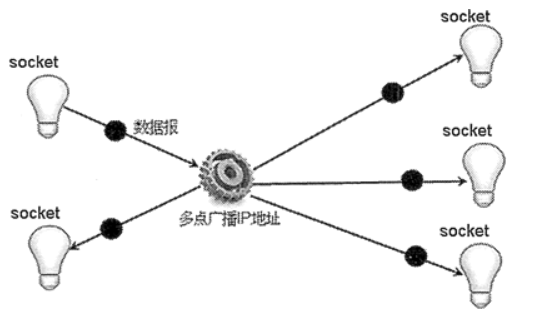
\includegraphics[scale=0.6]{fig1.png}}
\par{从上图中可以看出,当 socket 把一个数据报发送到多点广播 IP 地址时,该数据报将被自动广播到加入该地址的所有 socket。该 socket 既可以将数据报发送到多点广播地址,也可以接收其他主机的广播信息。
}

\subsection{winsock2介绍:}{WinSock2是连接系统和用户使用的软件之间用于交流的一个接口,这个功能就是修复软件与系统正确的通讯的作用。}
\par{Winsock2 SPI(Service Provider Interface)服务提供者接口建立在Windows开放系统架构WOSA(Windows Open System Architecture)之上,是Winsock系统组件提供的面向系统底层的编程接口。Winsock系统组件向上面向用户应用程序提供一个标准的API接口;向下在Winsock组件和Winsock服务提供者(比如TCP/IP协议栈)之间提供一个标准的SPI接口。各种服务提供者是Windows支持的DLL,挂载在Winsock2 的Ws2\_{}32.dll模块下。对用户应用程序使用的Winsock2 API中定义的许多内部函数来说,这些服务提供者都提供了它们的对应的运作方式(例如API函数WSAConnect有相应的SPI函数WSPConnect)。多数情况下,一个应用程序在调用Winsock2 API函数时,Ws2\_{}32.dll会调用相应的Winsock2 SPI函数,利用特定的服务提供者执行所请求的服务。}
\par{简单来说,winsock2为Windows系统提供了socket编程的底层架构,使用户可以在Windows系统下完成socket编程。}

\subsection{部分代码解析:}
\subsubsection{win\_{}re.cpp(接受端程序):}
\par\text{定义网络参数}
\par{
\begin{lstlisting}
#define MCASTADDR "234.5.6.7"
#define MCASTPORT 12345
#define BUFSIZE 1024
#define DEFAULT_COUNT 500
\end{lstlisting}
}

\par\text{套接字等变量}
\par{
\begin{lstlisting}
	WSADATA wsd;
	struct sockaddr_in local,
	remote,
	from;
	SOCKET sock, sockM;
	TCHAR recvbuf[BUFSIZE],
	sendbuf[BUFSIZE];
	int len = sizeof(struct sockaddr_in),
	optval,
	ret;
	DWORD i=0;
\end{lstlisting}
}

\text{绑定本地local socket}
\par{
\begin{lstlisting}
	local.sin_family=AF_INET;
	local.sin_port = htons(MCASTPORT);
	local.sin_addr.s_addr = dwInterface;
	
	if(bind(sock,(struct sockaddr *)&local ,sizeof(local))
			==SOCKET_ERROR){
		printf("bind failed with :%d \n", WSAGetLastError());
		closesocket(sock);
		WSACleanup();
		return -1;
	}

\end{lstlisting}
}

\text{加入多播组}
\par{
\begin{lstlisting}
	remote.sin_family =AF_INET;
	remote.sin_port = htons(iPort);
	remote.sin_addr.s_addr = dwMulticastGroup;
	if((sockM = WSAJoinLeaf(sock,(SOCKADDR *)&remote,
			sizeof(remote),NULL,NULL,NULL,NULL,JL_BOTH))
			==INVALID_SOCKET){
		printf("WSAJoinLeaf() failed : %d\n", WSAGetLastError());
		closesocket(sock);
		WSACleanup();
		return -1;
	}

\end{lstlisting}
}

\text{接受数据并输出}
\par{
\begin{lstlisting}
	printf("Start rece...\n");
	for(i = 0;i < dwCount;i++)
	{
		//printf("hhh");
		if((ret = recvfrom(sock,recvbuf,BUFSIZE,0, 
			(struct sockaddr *)&from , &len))
			==SOCKET_ERROR){
			printf("recvfrom failed with: %d\n" ,
					 WSAGetLastError());
			closesocket(sockM);
			closesocket(sock);
			WSACleanup();
			return -1;
		}
		
		recvbuf[ret] = 0;
		printf("RECV: '%s' from <%s>\n", recvbuf,
				 inet_ntoa(from.sin_addr));
	}
\end{lstlisting}
}
\subsubsection{win\_{}se.cpp(发送端程序):}
\par{对于网络设置部分,两个程序均采用了相同配置,所以此从只给出发送数据的部分代码。}
\par\text{发送数据}
\par{
\begin{lstlisting}
	printf("Start send...\n");
	for ( i = 0; i < dwCount; i++)
	{
		sprintf(sendbuf, "server 1: This is a test: %d", i);
		printf("%s\n", sendbuf);
		if (sendto(sock,(char *)sendbuf,strlen(sendbuf),0,
				(struct sockaddr *) &remote,
				sizeof(remote))
				==SOCKET_ERROR){
			printf("sendto failed with: %d\n", 
					WSAGetLastError());
			closesocket(sockM);
			closesocket(sock);
			WSACleanup();
			return -1;
		}
		Sleep(500);
	}
	
\end{lstlisting}
}
\section{实验结果与分析}
\par{首先给出程序的运行结果:\\}
\subsection{发送端结果:}
\par\centerline{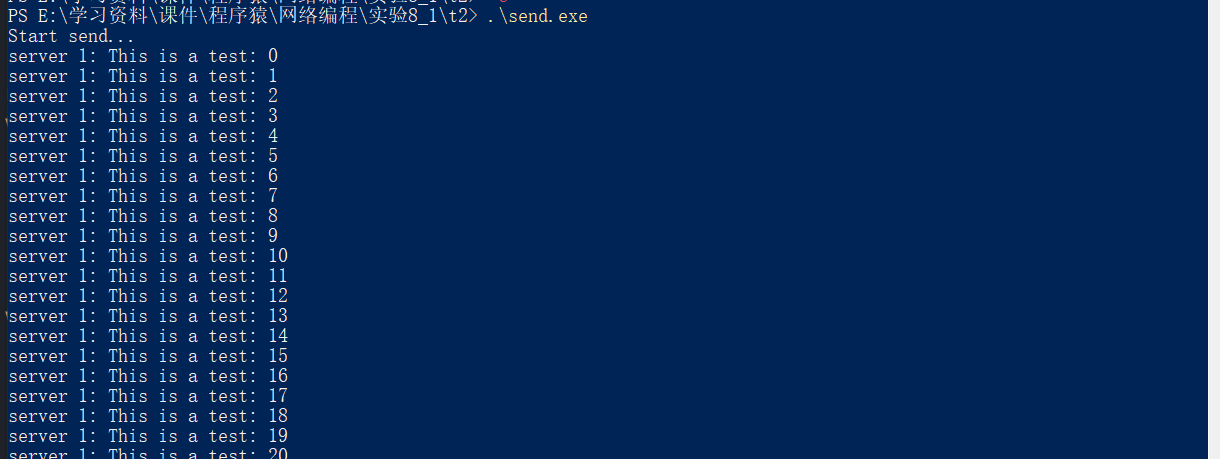
\includegraphics[scale=0.4]{fig3.png}}
\subsection{接收端结果:}
\par\centerline{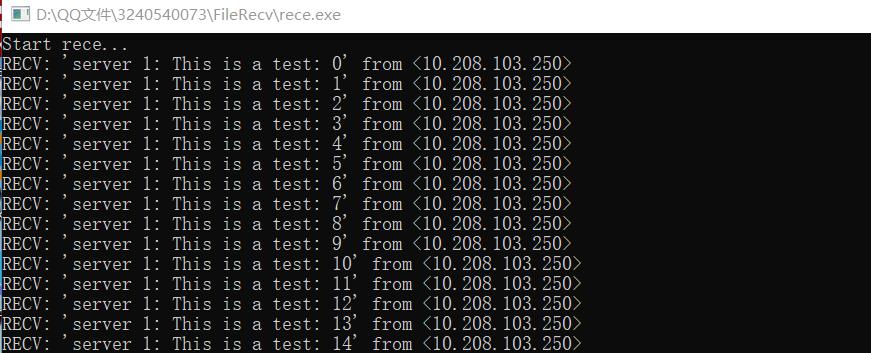
\includegraphics[scale=0.55]{fig2.png}}
\subsection{分析}

\par{从上方两个截图中可以清楚看到,发送端发出的报文数据,被接收端准确接收,因此,本次多播实验是一次成功的实验。}
\subsection{总结}
\par{通过本次实验,首先是了解了多播的原理与机制,再学习了winsock2的编程,掌握了Windows下的socket编程,本次实验过程中还涉及一些网络,网卡的配置,可谓是收获颇丰。}
\end{document}
